% # 5.3 同步操作和强制排序

假设两个线程,一个向数据结构中填充数据,另一个读取数据结构中的数据。为了避免恶性条件竞争,第一个线程设置一个标志,用来表明数据已经准备就绪,从而第二个线程在这个标志设置前不能读取数据。

代码5.2 不同线程对数据的读写

\begin{cpp}
#include <vector>
#include <atomic>
#include <iostream>

std::vector<int> data;
std::atomic<bool> data_ready(false);

void reader_thread()
{
  while(!data_ready.load())  // 1
  {
    std::this_thread::sleep(std::milliseconds(1));
  }
  std::cout<<"The answer="<<data[0]<<"\m";  // 2
}
void writer_thread()
{
  data.push_back(42);  // 3
  data_ready=true;  // 4
}
\end{cpp}

先把等待数据的循环①放在一边(因为每一个数据项都必须是原子的,所以这个循环不会在线程间产生数据共享)。当非原子读②和写③对同一数据结构进行无序访问时,破坏了循环遵守的访问顺序,所以会产生未定义行为。

访问顺序通过对\texttt{std::atomic<bool>}类型的data\_ready变量进行操作完成,这些操作通过\textit{\href{http://en.wikipedia.org/wiki/Happened-before}{先行}}(happens-before)和\textit{同发}(synchronizes-with)确定顺序。写入数据③在写入data\_ready④前发生,读取①发生在读取数据②之前。当data\_ready①为true,写操作就会与读操作同步,建立一个“先行”的关系。因为“先行”关系是可传递的,所以写入③先行于写入④,这两个行为又先行于读取操作①,之前的操作都先行于读取数据②,这样就强制了顺序:写入数据先行于读取数据。图5.2展示了“先行”关系在两线程间的重要性,读者线程的while循环中有一对迭代。

% ![](../../images/chapter5/5-2.png)
\begin{center}
    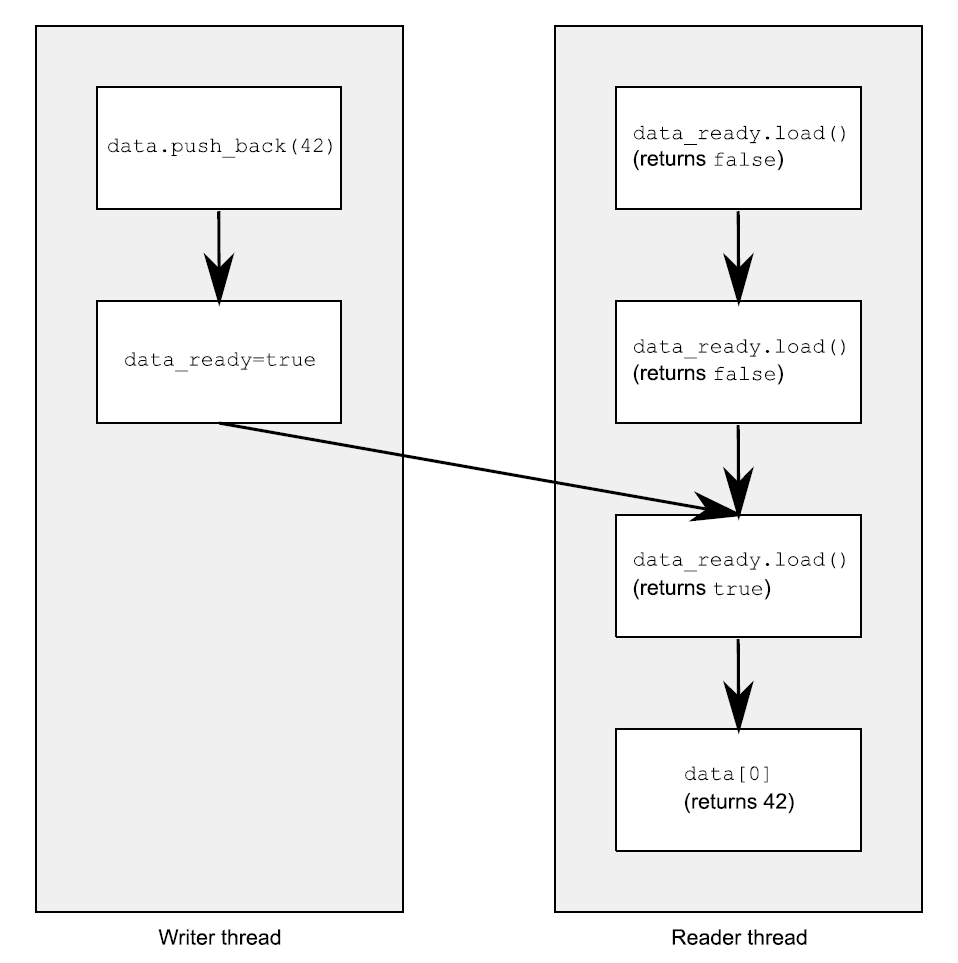
\includegraphics[width=0.7\textwidth]{content/chapter05/images/5-2.png}\\
    图5.2 对非原子操作,使用原子操作对操作进行强制排序
\end{center}

对一个值来说写操作必然先于读操作!默认都是原子操作时,这无疑是正确的(这就是原子操作为默认属性的原因)。不过,原子操作对于排序要求也有其他选项。

现在,来看看“先行”和“同发”操作的真正意义,先从“同步发生”开始说起。

\mySubsubsection{5.3.1}{同步发生}

“同发”只在原子类型之间进行。例如:操作一个数据结构(对互斥量上锁),如果数据结构包含有原子类型,并且操作内部执行了一定的原子操作,那这些操作就是“同发”关系。

“同发”的基本想法:原子写操作W对变量x进行标记,同步与对x进行原子读操作,读取的是W操作写入的内容,或是W之后,同一线程上的原子写操作对x写入的值,亦或是任意线程对x的一系列原子读-改-写操作(例如,fetch\_add()或compare\_exchange\_weak())。

因为对原子类型的操作默认都有“适当的标记”,如果线程A存储了一个值,并且线程B读取了这个值,线程A的存储操作与线程B的载入操作就是同步发生关系。

所有细微的差别都在“适当的标记”中,C++内存模型允许为原子类型提供各种约束顺序。

\mySubsubsection{5.3.2}{先行发生}

“先行”关系是一个程序中基本构建块的操作顺序:指定了某个操作去影响另一个操作。对于单线程来说:一个操作排在另一个之后,那这个操作就先执行。如果源码中操作A发生在操作B之前,那A就先行于B。可以回看代码5.2:对data的写入③先于对data\_ready④的写入。如果操作在同时发生,因为操作间无序执行,通常情况下就没有先行关系了。下面的程序会输出“1,2”或“2,1”,因为两个get\_num()的执行顺序未指定。

代码5.3 对于参数中的函数调用顺序未指定顺序

\begin{cpp}
#include <iostream>
void foo(int a,int b)
{
  std::cout<<a<<”,”<<b<<std::endl;
}
int get_num()
{
  static int i=0;
  return ++i;
}
int main()
{
  foo(get_num(),get_num());  // 无序调用get_num()
}
\end{cpp}

这种情况下,操作在单一声明中可测序,例如:逗号操作符的使用或是表达式的结果作为参数传给另一个表达式。通常情况下,操作在单一声明中不可排序,所以无法先行安排顺序(也就没有先行发生了)。

这只是对之前单线程排序的重述,放在这里有什么新意吗?新意在于线程间的互相作用:如果操作A在线程上,并且线程先行于另一线程上的操作B,那么A就先行于B。只是添加了一个新关系(线程间的先行),但在编写多线程程序时,这就是至关重要的关系了。

线程间的先行比较简单,并且依赖与同步关系(详见5.3.1节):如果操作A在一个线程上,与另一个线程上的操作B同步,那么A就线程间先行于B。这也是一个传递关系:如果A线程间先行于B,并且B线程间先行于C,那么A就线程间先行于C。

线程间先行可以与排序先行相结合:如果操作A排序先行于操作B,并且操作B线程间先行于操作C,那么A线程间先行于C。同样的,如果A同步于B,并且B排序先于C,那么A线程间先行于C。当对数据进行一系列修改(单线程)时,只需要对数据进行一次同步即可。

强先行发生关系会有一些不同,不过在大多数情况下是一样的。如果操作A与操作B同步,或操作A的顺序在操作B之前,那么A就是强先行于B。也适用于顺序传递:如果A强先行于B,并且B强先行于C,那么A就肯定强先行于C。事件在线程间的先行关系与普通事件有所区别,这里的区别就在于操作被标记为memory\_order\_consume(详见5.3.3节),但不是强先行关系。由于大多数代码并不适用memory\_order\_consume内存序,因此这种区别在实际中可能不会表现的很明显。为了描述方便,本书中使用”先行发生“对这种关系进行描述。

这些是线程间强制排序操作的关键规则,也是让代码5.2正常运行的因素。并在数据依赖上有细微的差别。为了理解这些差别,需要说一下原子操作使用的内存序,以及这些内存序和同步发生之间的联系。

\mySubsubsection{5.3.3}{原子操作的内存序}

这里有六个内存序列选项可应用于对原子类型的操作:

% 1. memory_order_relaxed
% 2. memory_order_consume
% 3. memory_order_acquire
% 4. memory_order_release
% 5. memory_order_acq_rel
% 6. memory_order_seq_cst

除非为特定的操作指定一个序列选项,要不内存序列默认都是memory\_order\_seq\_cst。

虽然有六个选项,但仅代表三种内存模型:顺序一致性(sequentially consistent),获取-释放序(memory\_order\_consume, memory\_order\_acquire, memory\_order\_release和memory\_order\_acq\_rel)和自由序(memory\_order\_relaxed)。

不同的内存序在不同的CPU架构下功耗不同,例如:基于处理器架构的可视化精细操作系统,可使用顺序一致或被获取-释放序(在自由序之前)添加的同步指令。如果有多个处理器,额外的同步指令会消耗大量的时间,从而降低系统性能。另一方面,CPU使用的是x86或x86-64架构(例如,使用Intel或AMD处理器的台式电脑),这种架构的CPU不需要对获取-释放序添加额外的指令(没有保证原子性的必要了),顺序一致序对于加载操作也不需要任何处理,但在进行存储时需要额外的消耗。

不同种类的内存序,允许使用其提升相关操作的性能。使用顺序一致序(相较于其他序列,它是最简单的)时,对于在通常情况来说就够用了。

\textbf{顺序一致性}

默认序命名为顺序一致性,因为程序中的行为从任意角度去看,序列都保持一定顺序。如果原子实例的所有操作都是序列一致的,那么多线程就会如单线程那样以某种特殊的排序执行。目前来看,该内存序是最容易理解的,这也是将其设置为默认的原因:不同的操作也要遵守相同的顺序。因为行为简单,可以使用原子变量进行编写。通过不同的线程,可以写出所有可能的操作消除那些不一致,以及确认代码的行为是否与预期相符。所以,操作都不能重排;如果代码在一个线程中,将一个操作放在另一个操作前面,那其他线程也需要了解这个顺序。

从同步的角度看,是对同一变量的存储操作与载入操作的同步。这就提供了一种对两个(以上)线程操作的排序约束,但顺序一致的功能要比排序约束大的多,所以对于使用顺序一致的原子操作,都会存储值后再加载,代码5.4就是这种一致性约束的演示。这种约束不是线程在自由序中使用原子操作,这些线程依旧可以知道操作以不同顺序排列,所以必须使用顺序一致的操作去保证,多线程下的加速效果。

不过,简单就要付出代价。多核机器会加强对性能的惩罚,因为整个序列中的操作都必须在多个处理器上保持一致,可能需要对处理器间的同步操作进行扩展(代价很昂贵!)。即便如此,一些处理器架构(比如:通用x86和x86-64架构)就提供了相对廉价的顺序一致性,所以需要考虑使用顺序一致性对性能的影响,就需要去查阅目标处理器的架构文档进行更多的了解。

以下代码展示了顺序一致性的行为,对于x和y的加载和存储都显示标注为memory\_order\_seq\_cst。因为是默认项,所以在这段代码中,标签可能会被忽略。

代码5.4 全序——序列一致性

\begin{cpp}
#include <atomic>
#include <thread>
#include <assert.h>

std::atomic<bool> x,y;
std::atomic<int> z;

void write_x()
{
  x.store(true,std::memory_order_seq_cst);  // 1
}

void write_y()
{
  y.store(true,std::memory_order_seq_cst);  // 2
}
void read_x_then_y()
{
  while(!x.load(std::memory_order_seq_cst));
  if(y.load(std::memory_order_seq_cst))  // 3
    ++z;
}
void read_y_then_x()
{
  while(!y.load(std::memory_order_seq_cst));
  if(x.load(std::memory_order_seq_cst))  // 4
    ++z;
}
int main()
{
  x=false;
  y=false;
  z=0;
  std::thread a(write_x);
  std::thread b(write_y);
  std::thread c(read_x_then_y);
  std::thread d(read_y_then_x);
  a.join();
  b.join();
  c.join();
  d.join();
  assert(z.load()!=0);  // 5
}
\end{cpp}

assert⑤语句是永远不会触发的,因为不是存储x的操作①发生,就是存储y的操作②发生。如果在read\_x\_then\_y中加载y③返回false,是因为存储x的操作发生在存储y的操作之前。在read\_y\_then\_x中加载x④必定会返回true,因为while循环能保证在某一时刻y是true。因为memory\_order\_seq\_cst的语义需要一个全序将所有操作都标记为memory\_order\_seq\_cst,这就暗示着“加载y并返回false③”与“存储y①”的操作,需要有一个确定的顺序。只有在全序时,当一个线程看到\texttt{x==true},随后又看到\texttt{y==false},这就说明在总序列中存储x的操作发生在存储y的操作之前。

因为事情都是对称的,所以有可能以其他方式发生,比如:加载x④的操作返回false,或强制加载y③的操作返回true。这两种情况下,z都等于1。当两个加载操作都返回true,z就等于2。所以任何情况下,z都不能是0。

当read\_x\_then\_y知道x为true,并且y为false时,这些操作就有“先行”关系了,如图5.3所示。

% ![](../../images/chapter5/5-3.png)
\begin{center}
    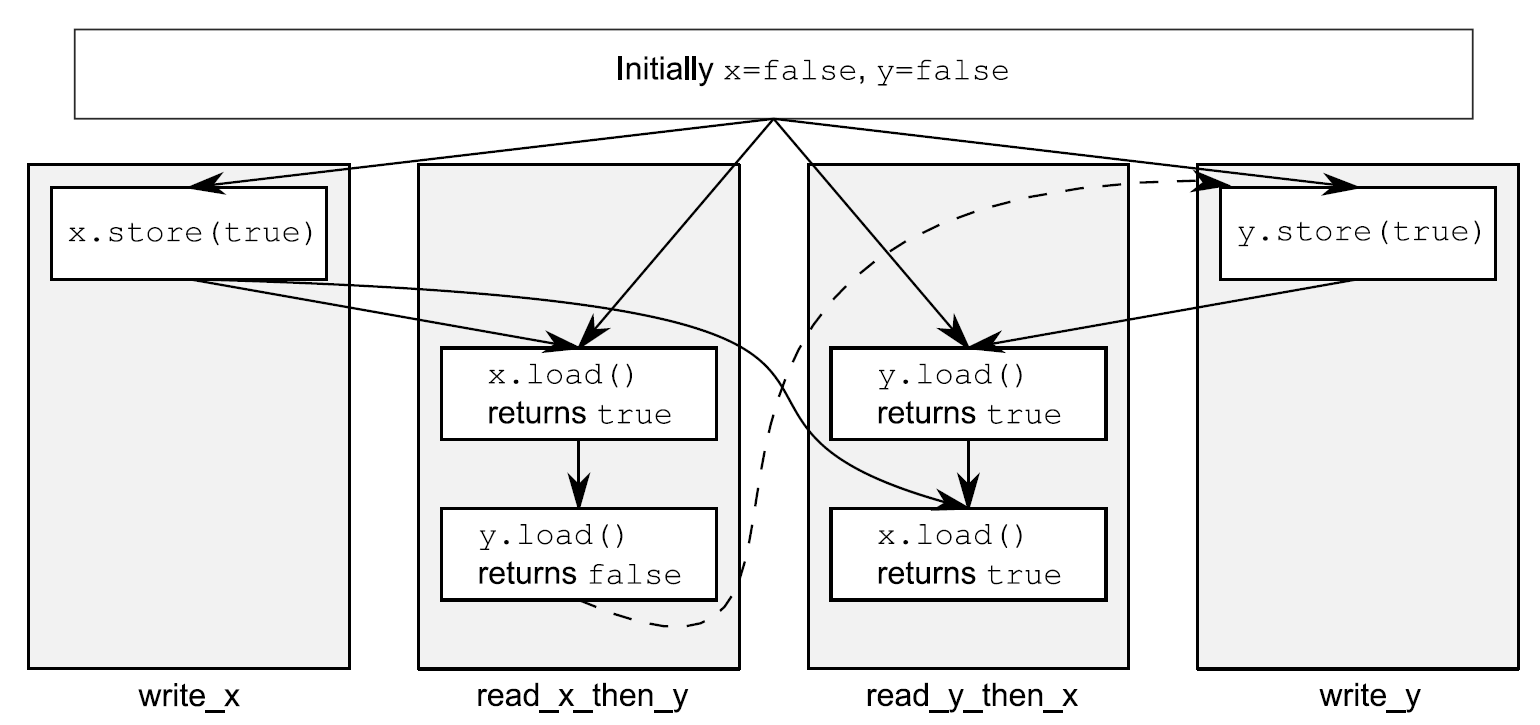
\includegraphics[width=0.7\textwidth]{content/chapter05/images/5-3.png}\\
    图5.3 序列一致与先行关系
\end{center}

虚线始于read\_x\_then\_y中对y的加载操作,到达write\_y中对y的存储,其表示排序关系需要保持一致:全局操作序memory\_order\_seq\_cst中,加载操作必须在存储操作前发生,这样就产生了图中的情况。

序列一致性是最简单、直观的序列,因为需要对所有线程进行全局同步,所以也是开销最大的内存序。多处理器设备上需要在处理期间,在信息交换上耗费大量的时间。

为了避免这种消耗,就需考虑使用其他内存序。

\textbf{非顺序一致性内存}

当踏出序列一致的世界时,事情就开始复杂了。不同线程看到相同操作,不一定有着相同的顺序,还有对于不同线程的操作,都会一个接着另一个执行的想法就不可行了。不仅是考虑事情同时发生的问题,还有线程没办法保证一致性。为了写出(或仅是了解)一段使用非默认内存序列的代码,绝不仅是编译器重新排列指令的事情。即使线程运行相同的代码,都能拒绝遵循事件发生的顺序,因为操作在其他线程上没有明确的顺序限制,不同的CPU缓存和内部缓冲区,在同样的存储空间中可以存储不同的值。这非常重要,这里再重申一次:线程没办法保证一致性。

不仅是要摒弃串行的想法,还要放弃编译器或处理器重排指令的想法。没有明确顺序限制时,就需要所有线程要对每个独立变量统一修改顺序。对不同变量的操作可以体现在不同线程的不同序列上,提供的值要与任意附加顺序限制保持一致。

踏出排序一致世界后,就使用memory\_order\_relaxed对所有操作进行约束。如果已经有所了解,可以跳到获取-释放序继续阅读,获取-释放序允许在操作间引入顺序关系。

\textbf{自由序}

原子类型上的操作以自由序执行。同一线程中对于同一变量的操作还是遵从先行关系,但不同线程不需要规定顺序。唯一的要求是在访问同一线程中的单个原子变量不能重排序,当给定线程看到原子变量的值时,随后线程的读操作就不会去检索较早的那个值。当使用memory\_order\_relaxed时,不需要任何额外的同步,对于每个变量的修改顺序只存在于线程间共享。

为了演示如何使用非限制操作,只需要两个线程。

代码5.5 非限制操作只有非常少的顺序要求

\begin{cpp}
#include <atomic>
#include <thread>
#include <assert.h>

std::atomic<bool> x,y;
std::atomic<int> z;

void write_x_then_y()
{
  x.store(true,std::memory_order_relaxed);  // 1
  y.store(true,std::memory_order_relaxed);  // 2
}
void read_y_then_x()
{
  while(!y.load(std::memory_order_relaxed));  // 3
  if(x.load(std::memory_order_relaxed))  // 4
    ++z;
}
int main()
{
  x=false;
  y=false;
  z=0;
  std::thread a(write_x_then_y);
  std::thread b(read_y_then_x);
  a.join();
  b.join();
  assert(z.load()!=0);  // 5
}
\end{cpp}

这次assert⑤可能会触发,因为加载x的操作④可能读取到false,即使加载y的操作③读取到true,并且存储x的操作①先发与存储y的操作②。x和y是两个不同的变量,所以没有顺序去保证每个操作产生相关值的可见性。

非限制操作对于不同变量可以重排序,只要服从任意的先行关系即可(比如,在同一线程中)。尽管,不同的存储/加载操作间有着先行关系,这里不是在一对存储/加载之间了,所以加载操作可以看到“违反”顺序的存储操作。

% ![](../../images/chapter5/5-4.png)
\begin{center}
    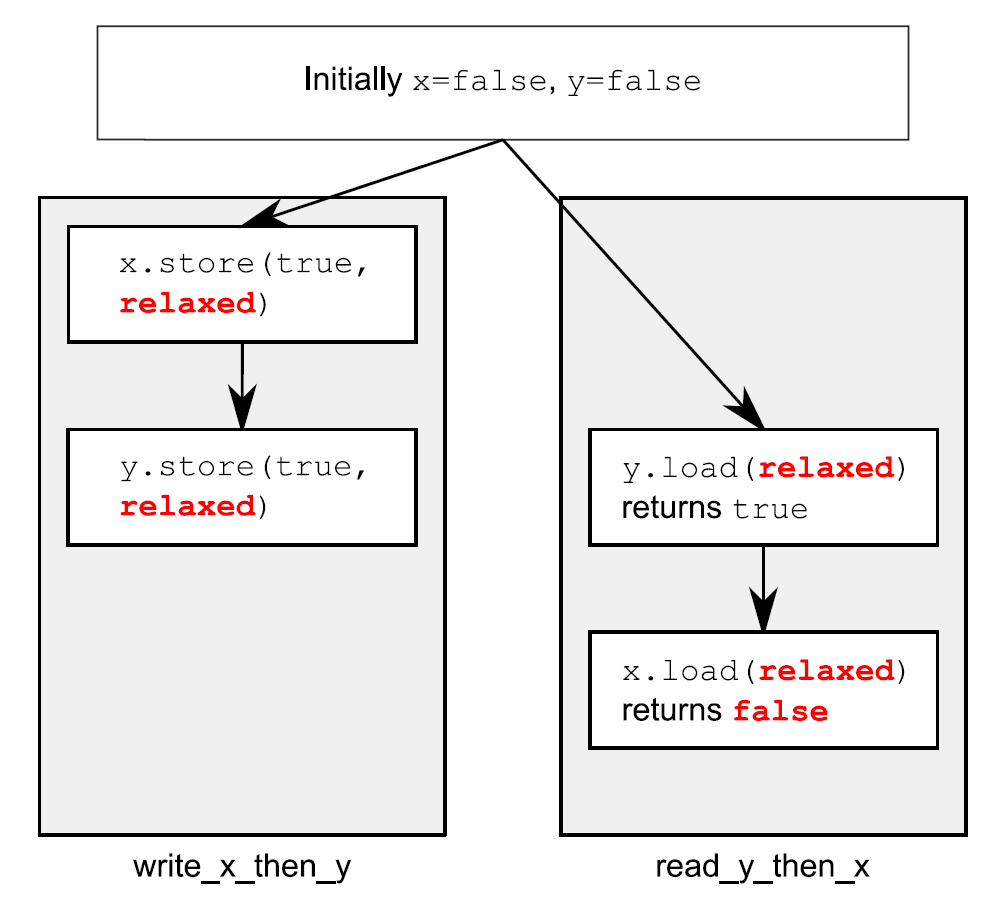
\includegraphics[width=0.7\textwidth]{content/chapter05/images/5-4.png}\\
    图5.4 非限制原子操作与先发执行
\end{center}

来看一个略微复杂的例子,有三个变量和五个线程。

代码5.6 非限制操作——多线程版

\begin{cpp}
#include <thread>
#include <atomic>
#include <iostream>

std::atomic<int> x(0),y(0),z(0);  // 1
std::atomic<bool> go(false);  // 2

unsigned const loop_count=10;

struct read_values
{
  int x,y,z;
};

read_values values1[loop_count];
read_values values2[loop_count];
read_values values3[loop_count];
read_values values4[loop_count];
read_values values5[loop_count];

void increment(std::atomic<int>* var_to_inc,read_values* values)
{
  while(!go)
    std::this_thread::yield();  // 3 自旋,等待信号
  for(unsigned i=0;i<loop_count;++i)
  {
    values[i].x=x.load(std::memory_order_relaxed);
    values[i].y=y.load(std::memory_order_relaxed);
    values[i].z=z.load(std::memory_order_relaxed);
    var_to_inc->store(i+1,std::memory_order_relaxed);  // 4
    std::this_thread::yield();
  }
}

void read_vals(read_values* values)
{
  while(!go)
    std::this_thread::yield(); // 5 自旋,等待信号
  for(unsigned i=0;i<loop_count;++i)
  {
    values[i].x=x.load(std::memory_order_relaxed);
    values[i].y=y.load(std::memory_order_relaxed);
    values[i].z=z.load(std::memory_order_relaxed);
    std::this_thread::yield();
  }
}

void print(read_values* v)
{
  for(unsigned i=0;i<loop_count;++i)
  {
    if(i)
      std::cout<<",";
    std::cout<<"("<<v[i].x<<","<<v[i].y<<","<<v[i].z<<")";
  }
  std::cout<<std::endl;
}

int main()
{
  std::thread t1(increment,&x,values1);
  std::thread t2(increment,&y,values2);
  std::thread t3(increment,&z,values3);
  std::thread t4(read_vals,values4);
  std::thread t5(read_vals,values5);

  go=true;  // 6 开始执行主循环的信号

  t5.join();
  t4.join();
  t3.join();
  t2.join();
  t1.join();

  print(values1);  // 7 打印最终结果
  print(values2);
  print(values3);
  print(values4);
  print(values5);
}
\end{cpp}

代码本质上很简单,三个全局原子变量①和五个线程。每一个线程循环10次,使用时memory\_order\_relaxed读取三个原子变量的值,并且将它们存储在一个数组上。其中三个线程每次通过循环④来更新其中一个原子变量,这时剩下的两个线程就负责读取。当线程都汇入主线程,就能打印出来每个线程存到数组上的值了。

原子变量go②用来确保线程同时退出。启动线程是昂贵的操作,并且没有明确的延迟,第一个线程可能在最后一个线程开始前结束。每个线程都在go变为true前,都在循环③⑤。并且当go设置为true时,所有线程都会开始运行⑥。

程序一种可能的输出为:

\begin{cpp}
(0,0,0),(1,0,0),(2,0,0),(3,0,0),(4,0,0),(5,7,0),(6,7,8),(7,9,8),(8,9,8),(9,9,10)
(0,0,0),(0,1,0),(0,2,0),(1,3,5),(8,4,5),(8,5,5),(8,6,6),(8,7,9),(10,8,9),(10,9,10)
(0,0,0),(0,0,1),(0,0,2),(0,0,3),(0,0,4),(0,0,5),(0,0,6),(0,0,7),(0,0,8),(0,0,9)
(1,3,0),(2,3,0),(2,4,1),(3,6,4),(3,9,5),(5,10,6),(5,10,8),(5,10,10),(9,10,10),(10,10,10)
(0,0,0),(0,0,0),(0,0,0),(6,3,7),(6,5,7),(7,7,7),(7,8,7),(8,8,7),(8,8,9),(8,8,9)
\end{cpp}

前三行中线程都做了更新,后两行线程只是做读取。每三个值都是一组x,y和z,并按照这样的顺序依次循环。对于输出,需要注意的是:

1. 第一组值中x增1,第二组值中y增1,第三组中z增1。
2. x元素只在给定集中增加,y和z也一样,但是是不均匀增加,并且每个线程中的相对顺序都不同。
3. 线程3看不到x或y的任何更新,它能看到的只有z的更新。这并不妨碍别的线程观察z的更新,并同时观察x和y的更新。

对于非限制操作,这个结果没毛病(但是不是唯一合法的输出)。任意组都用三个变量保持一致,从0到10依次递增,并且线程对相应变量进行递增操作,所以打印出的值在0到10的范围内都合理。

\textbf{了解自由序}

为了了解自由序是如何工作的,可先将每一个变量想象成在一个独立房间中拿着记事本的人。他的记事本上是一组值的列表,可以通过打电话的方式让他给你一个值,或让他写下一个新值。如果告诉他写下一个新值,他会将这个新值写在表的最后。如果让他给你一个值,他会从列表中读取一个值给你。

第一次与这人交谈时,如果问他要一个值,他可能会在现有的列表中选区任意值告诉你。如果之后再问他要一个值,可能会得到与之前相同的值,或是列表下端的其他值,他不会给你列表上端的值。如果让他写一个值,并且随后再问他要一个值,他要不就给你你刚告诉他的那个值,要不就是一个列表下端的值。

试想当他的笔记本上开始有5,10,23,3,1,2这几个数。如果问他索要一个值,你可能获取这几个数中的任意一个。如果他给你10,那么下次再问他要值的时候可能会再给你10,或者10后面的数,但绝对不会是5。如果那你问他要了五次,他就可能回答“10,10,1,2,2”。如果你让他写下42,他将会把这个值添加在列表的最后。如果你再问他要值,他可能会告诉你“42”,直到有其他值写在了后面,并且他愿意将那个数告诉你。

现在,你有个朋友叫Carl,他也有那个计数员的电话。Carl也可以打电话给计算员,让他写下一个值或获取一个值,他对Carl回应的规则和你是一样的。他只有一部电话,所以一次只能处理一个人的请求,所以他记事本上的列表是一个简单的列表。但是,你让他写下一个新值的时候,不意味着他会将这个消息告诉Carl,反之亦然。如果Carl从他那里获取一个值“23”,之后因为你告诉他写下42,这不意味着下次他会将这件事告诉Carl。他可能会告诉Carl任意一个值,23,3,1,2,42亦或是67(是Fred在你之后告诉他的)。他会很高兴的告诉Carl“23,3,3,1,67”,与你告诉他的值完全不一致,这就像在使用便签跟踪告诉每个人的数字,如图5.5。

% ![](../../images/chapter5/5-5.png)
\begin{center}
    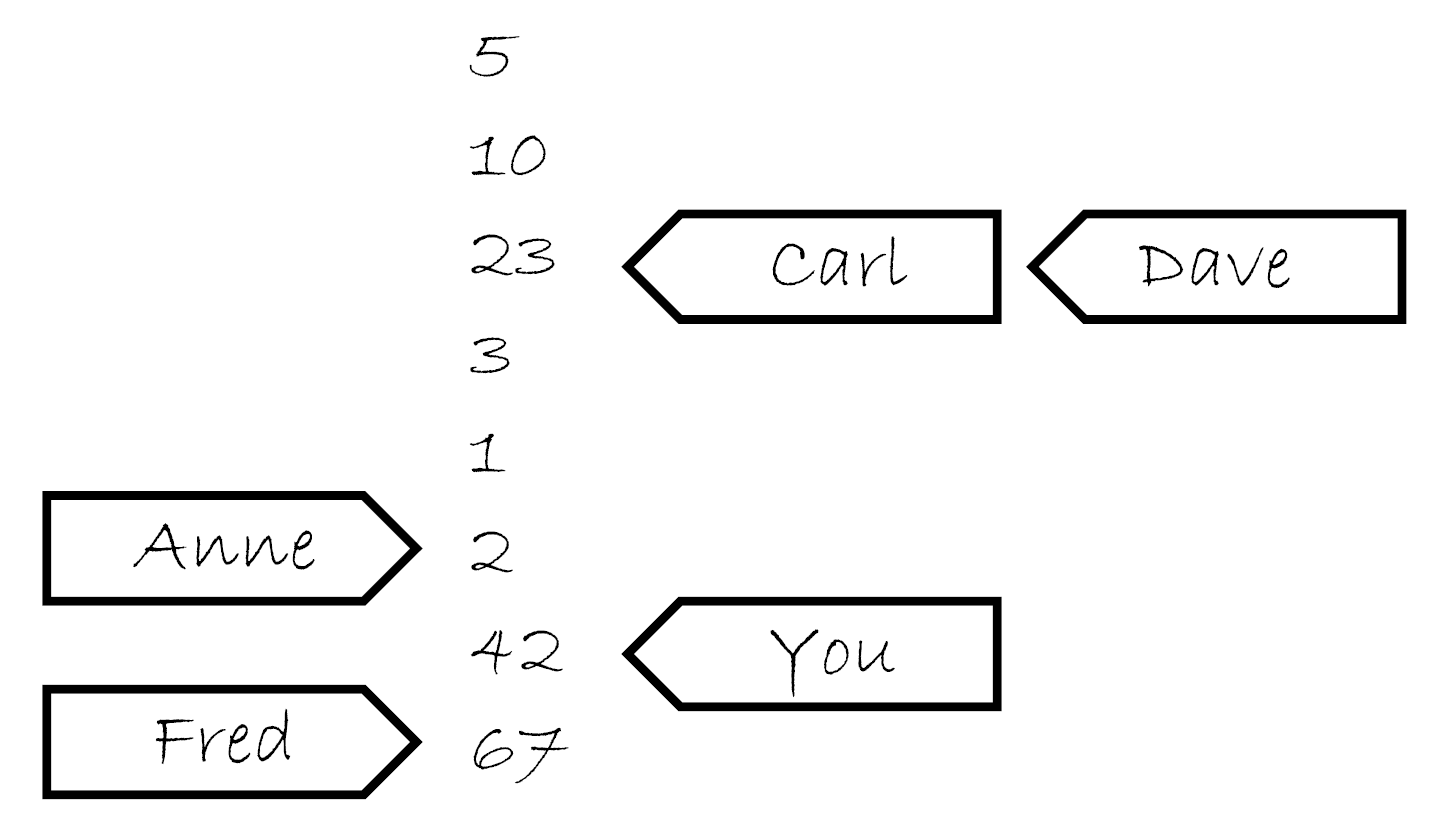
\includegraphics[width=0.7\textwidth]{content/chapter05/images/5-5.png}\\
    图5.5 计数员的笔记
\end{center}

现在,不仅仅有一个人在房间里,而是在一个小农场里,每个人都有一部电话和一个笔记本,这就是原子变量。每一个变量拥有自己的修改顺序(笔记上的简单数值列表),但是每个原子变量之间没有任何关系。如果每一个调用者(你,Carl,Anne,Dave和Fred)是一个线程,对每个操作使用memory\_order\_relaxed就会得到上面的结果。还有些事情可以告诉小房子里的人,例如:“写下这个值,并且告诉我现在列表中的最后一个值”(exchange),或“写下这个值,当列表的最后一个值为某值时,会进行猜测,如果猜错了,则告诉我最后一个值是多少”(compare\_exchange\_strong),这些都不影响一般性原则。

仔细回顾下代码5.5的逻辑,write\_x\_then\_y就像某人打电话给房子x里的人,并且告诉他写下true,之后打电话给y房间的另一个人,告诉他写下true。线程反复执行调用read\_y\_then\_x,就像打电话给房间y的人问他要值,直到要到true,然后打电话给房间x的,继续问他要值。在x房间中的人有义务告诉他列表中任意指定的值,所以他也是有权利说false。

这就让自由的原子操作变得难以处理,他们必须与原子操作结合使用,这些原子操作必须有较强的排序语义。为了让内部线程同步变得更有用,我强烈建议避免自由序的原子操作,除非它们是硬性要求的,并且使用时需要十二分的谨慎。如同代码5.5中使用双线程和双变量一样,不难想象在更多线程和更多变量的情况下,会变的多么复杂。

要想获取额外的同步,且不使用全局排序一致,可以使用\textit{获取-释放序}(acquire-release ordering)。

\textbf{获取-释放序}

这是\textit{自由序}(relaxed ordering)的加强版,虽然操作依旧没有统一顺序,但引入了同步。这种序列模型中,原子加载就是\textit{获取}(acquire)操作(memory\_order\_acquire),原子存储就是\textit{释放}(memory\_order\_release)操作,原子读-改-写操作(例如fetch\_add()或exchange())在这里,不是“获取”就是“释放”,或者两者兼有的操作(memory\_order\_acq\_rel),同步在线程释放和获取间是\textit{成对的}(pairwise),释放操作与获取操作同步就能读取已写入的值。下面列表中是使用获取-释放序(而非序列一致方式),对代码5.4的一次重写。

代码5.7 获取-释放不意味着统一操作顺序

\begin{cpp}
#include <atomic>
#include <thread>
#include <assert.h>

std::atomic<bool> x,y;
std::atomic<int> z;
void write_x()
{
  x.store(true,std::memory_order_release);
}
void write_y()
{
  y.store(true,std::memory_order_release);
}
void read_x_then_y()
{
  while(!x.load(std::memory_order_acquire));
  if(y.load(std::memory_order_acquire))  // 1
    ++z;
}
void read_y_then_x()
{
  while(!y.load(std::memory_order_acquire));
  if(x.load(std::memory_order_acquire))  // 2
    ++z;
}
int main()
{
  x=false;
  y=false;
  z=0;
  std::thread a(write_x);
  std::thread b(write_y);
  std::thread c(read_x_then_y);
  std::thread d(read_y_then_x);
  a.join();
  b.join();
  c.join();
  d.join();
  assert(z.load()!=0); // 3
}
\end{cpp}

例子中断言③可能会触发(就如同自由排序那样),因为在加载x②和y①时,可能读取到false。因为x和y是由不同线程写入,所以序列中的每一次释放和获取都不会影响到其他线程的操作。

图5.6展示了代码5.7的先行关系,对于读取的结果,两个(读取)线程看到的是两个完全不同的世界。如前所述,这可能是因为这里没有对先行顺序进行强制规定导致的。

% ![](../../images/chapter5/5-6.png)

\begin{center}
    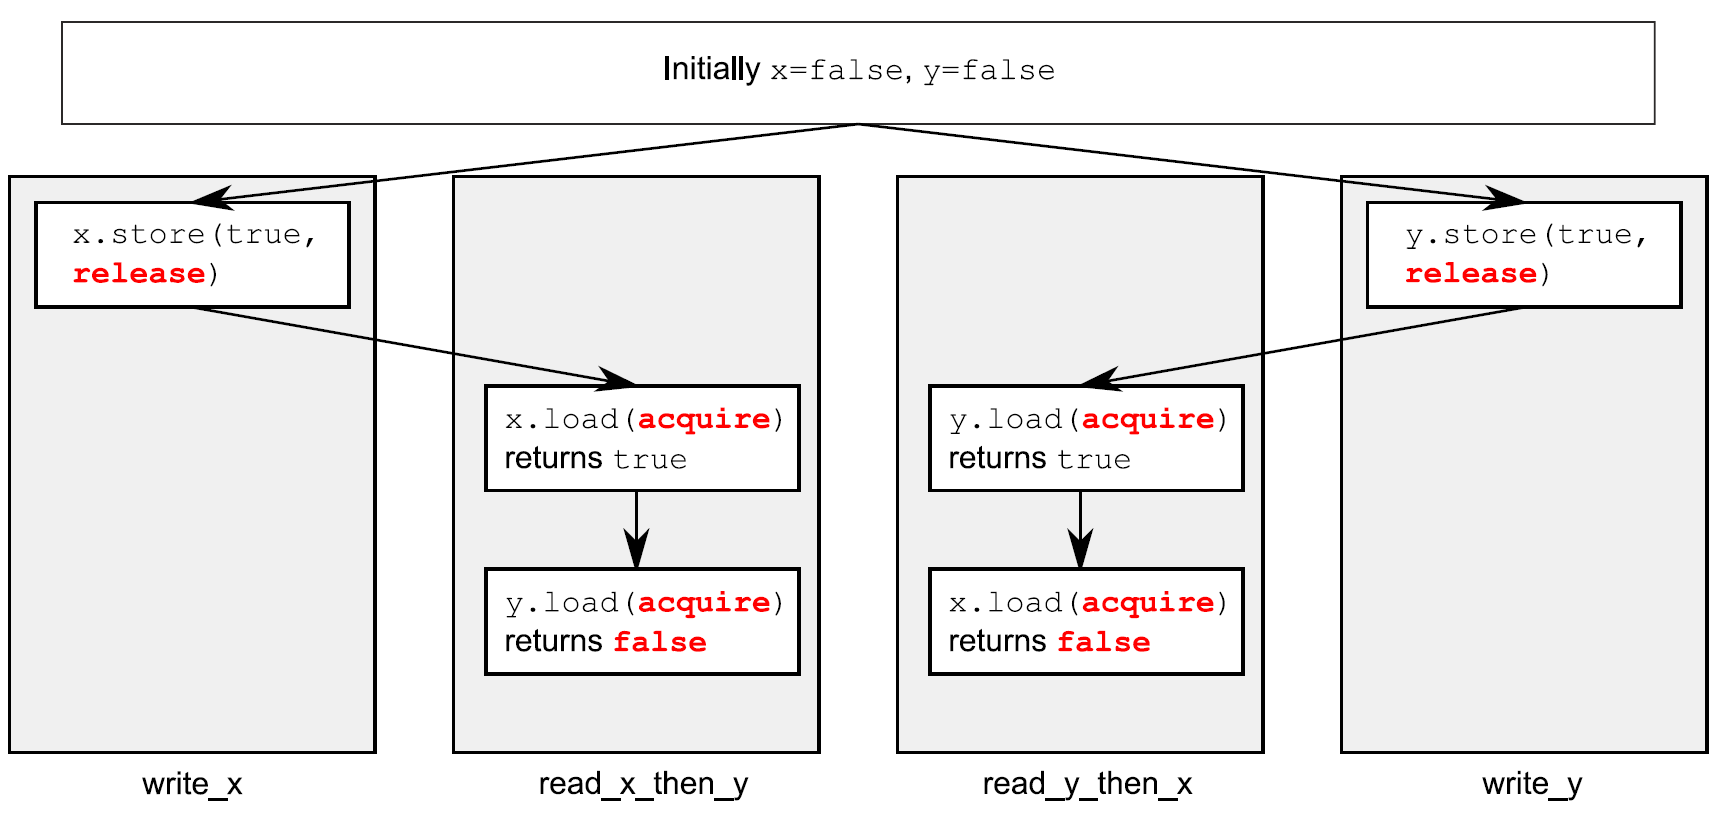
\includegraphics[width=0.7\textwidth]{content/chapter05/images/5-6.png}\\
    图5.6 获取-释放,以及先行过程
\end{center}

为了了解获取-释放序的优点,需要考虑将两次存储由一个线程来完成,就像代码5.5那样。当需要使用memory\_order\_release改变y中的存储,并使用memory\_order\_acquire来加载y中的值,而后就会影响对x的操作。

代码5.8 获取-释放序操作会影响释放操作

\begin{cpp}
#include <atomic>
#include <thread>
#include <assert.h>

std::atomic<bool> x,y;
std::atomic<int> z;

void write_x_then_y()
{
  x.store(true,std::memory_order_relaxed);  // 1
  y.store(true,std::memory_order_release);  // 2
}
void read_y_then_x()
{
  while(!y.load(std::memory_order_acquire));  // 3 自旋,等待y被设置为true
  if(x.load(std::memory_order_relaxed))  // 4
    ++z;
}
int main()
{
  x=false;
  y=false;
  z=0;
  std::thread a(write_x_then_y);
  std::thread b(read_y_then_x);
  a.join();
  b.join();
  assert(z.load()!=0);  // 5
}
\end{cpp}

最后,读取y③时会得到true,和存储时写入的一样②。存储使用的是memory\_order\_release,读取使用的是memory\_order\_acquire,存储与读取就同步了。因为这两个操作是由同一个线程串行完成的,所以存储x①的操作先行于存储y②的操作。对y的存储同步与对y的加载,存储x也就先行于对y的加载,并且扩展先行于x的读取。因此,加载x的值必为true,并且断言⑤不会触发。如果对于y的加载不是在while循环中,情况可能就会有所不同。加载y的时候可能会读取到false,这种情况下对于读取到的x是什么值没有要求了。为了保证同步,加载和释放操作必须成对。所以,无论有何影响,释放操作存储的值必须要让获取操作看到。当存储②或加载③都是一个释放操作时,对x的访问就无序了,也就无法保证④处读到的是true,并且还会触发断言。

也可以将获取-释放序与之前提到记录员相关联,这样就需要添加很多东西到模型中。首先,每个存储操作做一部分更新,当你联系一个人时,让他写下一个数字,也需要告诉他更新哪一部分:“请在423组中写下99”。对于某一组的最后一个值的存储,你也需要告诉那个人:“请写下147,这是最后存储在423组的值”。隔间中的人会及时写下这一信息,并注明这个值的来源,这个就是存储-释放操作的模型。下一次,你告诉另外一个人写下一组值时,需要改变组号:“请在424组中写入41”

当你询问时就要做出一个选择:要不就仅仅询问一个值(这就是次自由加载,这种情况下,隔间中的人会给你的),要不就询问一个值以及其关于组的信息(是否是某组中的最后一个,这就是加载-获取模型)。当你询问组信息,且值不是组中的最后一个,隔间中的人会这样告诉你,“这个值是987,它是一个普通值”,但当这个值是最后一个时,他会告诉你:“数字为987,这个值是956组的最后一个,来源于Anne”。这样,获取-释放的语义就很明确了:当查询一个值,你告诉他所有组后,他会低头查看列表,看你给的这些数是不是在对应组的最后,并且告诉你那个值的属性,或继续在列表中查询。

如何理解模型中获取-释放的语义?首先,线程a运行write\_x\_then\_y函数,然后告诉在x屋的记录员,“请写下true作为组1的一部分,信息来源于线程a”,之后记录员工整的写下了这些信息。而后,线程a告诉在y屋的记录员,“请写下true作为组1的一部分,信息来源于线程a”。期间,线程b运行read\_y\_then\_x。线程b持续向y屋的记录员询问值与组的信息,直到它听到记录员说“true”。记录员可能需要告诉他很多遍,不过最终记录员还是说了“true”。y屋的记录员不仅仅是说“true”,他还要说“组1最后是由线程a写入”。

现在,线程b会持续询问x屋的记录员,但这次他会说“请给我一个值,我知道这个值是组1的值,并且是由线程a写入的”。所以现在,x屋中的记录员就开始查找组1中由线程a写入的值。这里他注意到,他写入的值是true,同样也是他列表中的最后一个值,所以必须读出这个值。否则,他将打破这个游戏的规则。

回看5.3.2节中对“线程间先行”的定义,一个很重要的特性就是可传递:当A线程间先行于B,并且B线程间先行于C,那么A就线程间先行于C。获取-释放序列可以在若干线程间使用同步数据,甚至在“中间”线程接触到这些数据前,使用这些数据。

\textbf{获取-释放序传递同步}

为了考虑传递顺序,至少需要三个线程。第一个线程用来修改共享变量,第二个线程使用“加载-获取”读取由“存储-释放”操作过的变量,并且再对第二个变量进行“存储-释放”操作。最后,由第三个线程通过“加载-获取”读取第二个共享变量,并提供“加载-获取”操作来读取被“存储-释放”操作写入的值。为了保证同步关系,即便是中间线程没有对共享变量做任何操作,第三个线程也可以读取第一个线程操作过的变量。

代码5.9 使用获取和释放序传递同步

\begin{cpp}
std::atomic<int> data[5];
std::atomic<bool> sync1(false),sync2(false);

void thread_1()
{
  data[0].store(42,std::memory_order_relaxed);
  data[1].store(97,std::memory_order_relaxed);
  data[2].store(17,std::memory_order_relaxed);
  data[3].store(-141,std::memory_order_relaxed);
  data[4].store(2003,std::memory_order_relaxed);
  sync1.store(true,std::memory_order_release);  // 1.设置sync1
}

void thread_2()
{
  while(!sync1.load(std::memory_order_acquire));  // 2.直到sync1设置后,循环结束
  sync2.store(true,std::memory_order_release);  // 3.设置sync2
}
void thread_3()
{
  while(!sync2.load(std::memory_order_acquire));   // 4.直到sync1设置后,循环结束
  assert(data[0].load(std::memory_order_relaxed)==42);
  assert(data[1].load(std::memory_order_relaxed)==97);
  assert(data[2].load(std::memory_order_relaxed)==17);
  assert(data[3].load(std::memory_order_relaxed)==-141);
  assert(data[4].load(std::memory_order_relaxed)==2003);
}
\end{cpp}

尽管thread\_2只接触到变量syn1②和sync2③,对于thread\_1和thread\_3的同步就足够了,这能保证断言不会触发。首先,thread\_1将数据存储到data中先行于存储sync1①(它们在同一个线程内)。因为加载sync1①的是一个while循环,它最终会看到thread\_1存储的值。因此,对于sync1的存储先行于最终对于sync1的加载(在while循环中)。thread\_3的加载操作④,位于存储sync2③操作的前面。存储sync2③因此先行于thread\_3的加载④,加载又先行于存储sync2③,存储sync2又先行于加载sync2④,加载syn2又先行于加载data。因此,thread\_1存储数据到data的操作先行于thread\_3中对data的加载,并且保证断言都不会触发。

这个例子中,可将sync1和sync2通过在thread\_2中使用“读-改-写”操作(memory\_order\_acq\_rel)合并成一个独立的变量。其中会使用compare\_exchange\_strong()来保证thread\_1对变量只进行一次更新:

\begin{cpp}
std::atomic<int> sync(0);
void thread_1()
{
  // ...
  sync.store(1,std::memory_order_release);
}

void thread_2()
{
  int expected=1;
  while(!sync.compare_exchange_strong(expected,2,
              std::memory_order_acq_rel))
    expected=1;
}
void thread_3()
{
  while(sync.load(std::memory_order_acquire)<2);
  // ...
}
\end{cpp}

使用“读-改-写”操作,选择语义就很重要了。例子中,想要同时进行获取和释放的语义,所以memory\_order\_acq\_rel是一个不错的选择,但也可以使用其他内存序。即使存储了一个值,使用memory\_order\_acquire语义的fetch\_sub不会和任何东西同步的,因为没有释放操作。同样,使用memory\_order\_release语义的fetch\_or也不会和任何存储操作进行同步,因为对于fetch\_or的读取,并不是一个获取操作。使用memory\_order\_acq\_rel语义的“读-改-写”操作,每一个动作都包含获取和释放操作,所以可以和之前的存储操作进行同步,并且可以对随后的加载操作进行同步,就像上面例子一样。

如果将获取-释放和序列一致进行混合,“序列一致”的加载动作就如使用了获取语义的加载操作,序列一致的存储操作就如使用了释放语义的存储,“序列一致”的读-改-写操作行为就如使用了获取和释放的操作。“自由操作”依旧那么自由,但其会和额外的同步进行绑定(也就是使用“获取-释放”的语义)。

尽管结果并不那么直观,每个使用锁的同学都需要了解:锁住互斥量是一个获取操作,并且解锁这个互斥量是一个释放操作。随着互斥量的增多,必须确保同一个互斥量在读取变量或修改变量时上锁,所以获取和释放操作必须在同一个变量上,以保证访问顺序。当互斥量保护数据时,因为锁住与解锁的操作都是序列一致的操作,就保证了结果一致。当对原子变量使用获取和释放序时,代码必然会使用锁,即使内部操作序不一致,其外部表现将会为序列一致。

当原子操作不需要严格的序列一致序时,可以提供成对同步的获取-释放序,这种比全局序列一致性的成本更低,且有同步操作。为了保证序列能够正常的工作,这里还需要一些权衡,还要保证隐式的跨线程行为是没有问题的。

\textbf{获取-释放序和memory\_order\_consume的数据相关性}

介绍本章节的时候,说过memory\_order\_consume是“获取-释放”模型的一部分,但并没有对其进行过多的讨论。因为memory\_order\_consume很特别:完全依赖于数据,并且其展示了与线程间先行关系(可见5.3.2节)的不同之处。这个内存序非常特殊,即使在C++17中也不推荐使用。这里只为了完整的覆盖内存序而讨论, memory\_order\_consume不应该出现在代码中。

数据依赖的概念相对简单:第二个操作依赖于第一个操作的结果,这样两个操作之间就有了数据依赖。这里有两种新关系用来处理数据依赖:\textit{前序依赖}(dependency-ordered-before)和\textit{携带依赖}(carries-a-dependency-to)。携带依赖对于数据依赖的操作,严格应用于一个独立线程和其基本模型。如果A操作结果要使用操作B的操作数,则A将携带依赖于B。如果A操作的结果是一个标量(比如int),而后的携带依赖关系仍然适用于,当A的结果存储在一个变量中,并且这个变量需要被其他操作使用。这个操作可以传递,所以当A携带依赖B,并且B携带依赖C,就可以得出A携带依赖C的关系。

当不影响线程间的先行关系时,对于同步来说没有任何好处:当A前序依赖B,那么A线程间也前序依赖B。

这种内存序在原子操作载入指向数据的指针时很重要,当使用memory\_order\_consume作为加载语义,并且memory\_order\_release作为存储语义时,就要保证指针指向的值已同步,并且不要求其他非独立数据同步。

代码5.10 使用\texttt{std::memroy\_order\_consume}同步数据

\begin{cpp}
struct X
{
int i;
std::string s;
};

std::atomic<X*> p;
std::atomic<int> a;

void create_x()
{
  X* x=new X;
  x->i=42;
  x->s="hello";
  a.store(99,std::memory_order_relaxed);  // 1
  p.store(x,std::memory_order_release);  // 2
}

void use_x()
{
  X* x;
  while(!(x=p.load(std::memory_order_consume)))  // 3
    std::this_thread::sleep(std::chrono::microseconds(1));
  assert(x->i==42);  // 4
  assert(x->s=="hello");  // 5
  assert(a.load(std::memory_order_relaxed)==99);  // 6
}

int main()
{
  std::thread t1(create_x);
  std::thread t2(use_x);
  t1.join();
  t2.join();
}
\end{cpp}

尽管,存储a①在存储p②之前,并且存储p的操作标记为memory\_order\_release,加载p③的操作标记为memory\_order\_consume,所以存储p仅先行那些需要加载p的操作。因为对x变量操作的表达式对加载p的操作携带有依赖,所以X结构体中数据成员所在的断言语句④⑤不会被触发。另一方面,对于加载变量a⑥的断言就不能确定是否能触发,因为这个操作标记为memory\_order\_relaxed,所以这个操作并不依赖于p的加载操作,也无法保证已经读取数据。

有时,不想为携带依赖增加其他开销。想使用编译器在寄存器中缓存这些值,以及优化重排序操作代码。可以使用\texttt{std::kill\_dependecy()}显式打破依赖链,\texttt{std::kill\_dependency()}是一个简单的函数模板,会复制提供的参数给返回值。例如,一个全局的只读数组,当其他线程对数组索引进行检索时,使用的是\texttt{std::memory\_order\_consume},可以使用\texttt{std::kill\_dependency()}让编译器知道这里不需要重新读取该数组的内容。

\begin{cpp}
int global_data[]={ … };
std::atomic<int> index;

void f()
{
  int i=index.load(std::memory_order_consume);
  do_something_with(global_data[std::kill_dependency(i)]);
}
\end{cpp}

实际操作中,应该使用memory\_order\_acquire,而不是memory\_order\_consume和\texttt{std::kill\_dependency}。

现在,已经讨论了所有的内存序,是时候看看更加复杂的同步关系了——释放队列。

\mySubsubsection{5.3.4}{释放队列与同步}

回到5.3.1节,通过线程在存储和加载操作之间有(有序的)多个“读-改-写”操作(所有操作都已经做了适当的标记),所以可以获取原子变量存储与加载的同步关系。存储操作标记为memory\_order\_release,memory\_order\_acq\_rel或memory\_order\_seq\_cst,加载标记为memory\_order\_consum,memory\_order\_acquire或memory\_order\_sqy\_cst,并且操作链上的每一加载操作都会读取之前操作写入的值,因此链上的操作构成了一个释放序列(\textit{release sequence}),并且初始化存储同步(对应memory\_order\_acquire或memory\_order\_seq\_cst)或是前序依赖(对应memory\_order\_consume)的最终加载,操作链上的任何原子“读-改-写”操作可以拥有任意个内存序(甚至是memory\_order\_relaxed)。

为了了解这些操作的作用和其重要性,这里假设使用\texttt{atomic<int>}对共享队列的元素进行计数:

代码5.11 使用原子操作从队列中读取数据

\begin{cpp}
#include <atomic>
#include <thread>

std::vector<int> queue_data;
std::atomic<int> count;

void populate_queue()
{
  unsigned const number_of_items=20;
  queue_data.clear();
  for(unsigned i=0;i<number_of_items;++i)
  {
    queue_data.push_back(i);
  }

  count.store(number_of_items,std::memory_order_release);  // 1 初始化存储
}

void consume_queue_items()
{
  while(true)
  {
    int item_index;
    if((item_index=count.fetch_sub(1,std::memory_order_acquire))<=0)  // 2 一个“读-改-写”操作
    {
      wait_for_more_items();  // 3 等待更多元素
      continue;
    }
    process(queue_data[item_index-1]);  // 4 安全读取queue_data
  }
}

int main()
{
  std::thread a(populate_queue);
  std::thread b(consume_queue_items);
  std::thread c(consume_queue_items);
  a.join();
  b.join();
  c.join();
}
\end{cpp}

一种处理方式是让线程产生数据,并存储到一个共享内存中,而后调用count.store(number\_of\_items, memory\_order\_release)①让其他线程知道数据是可用的。线程群会消耗队列中的元素,调用count.fetch\_sub(1, memory\_order\_acquire)②后,从队列中获取元素。在这之前,需要对共享内存进行完整的读取④。一旦count归零,队列中就没有元素了,这时线程必须等待③。

只有带有memory\_order\_release语义,所以存储与加载同步,线程可以从缓存中读取元素。当有两个读取线程时,第二个fetch\_sub()操作将看到第一个线程修改的值,且没有值通过store写入其中。先不管释放序列的规则,第二个线程与第一个线程不存在先行关系,并且对共享内存中值的读取也不安全。除非第一个fetch\_sub()是带有memory\_order\_release语义,为两个消费者线程建立了不必要的同步。无论是释放序列的规则,还是具有memory\_order\_release语义的fetch\_sub操作,第二个消费者看到的是一个空的queue\_data,无法从其获取任何数据,并且还会产生条件竞争。幸运的是,第一个fetch\_sub()对释放顺序做了一些事情,所以store()能同步与第二个fetch\_sub()操作。两个消费者线程间不需要同步关系。过程在图5.7中展示,其中虚线表示的就是释放顺序,实线表示的是先行关系。

% ![](../../images/chapter5/5-7.png)

\begin{center}
    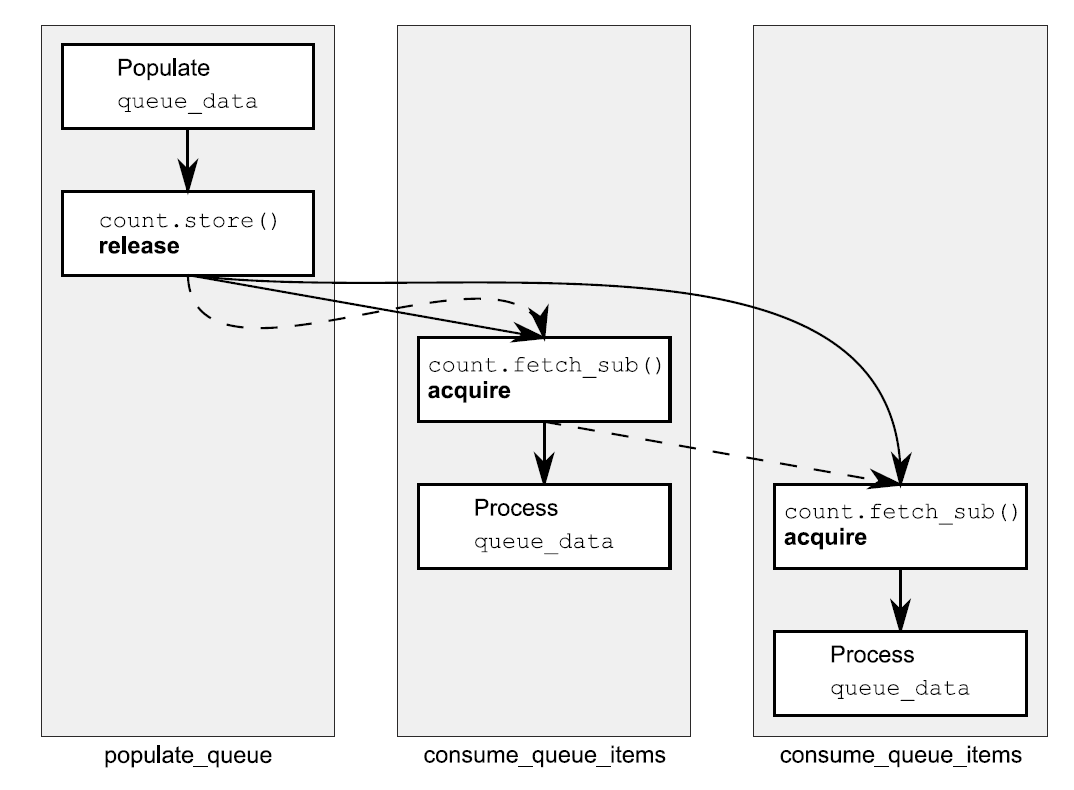
\includegraphics[width=0.7\textwidth]{content/chapter05/images/5-7.png}\\
    图5.7 代码5.11中对队列操作的释放顺序
\end{center}

操作链中可以有任意数量的链接,提供的都是“读-改-写”操作,比如fetch\_sub(),store(),每一个都会与使用memory\_order\_acquire语义的操作进行同步。例子中所有链接都是一样的,并且都是获取操作,但它们可由不同内存序列语义组成的操作混合。

虽然,大多数同步关系是对原子变量的操作应用了内存序,但这里依旧有必要介绍对排序的约束——栅栏(\textit{fences})。

\mySubsubsection{5.3.5}{栅栏}

栅栏操作会对内存序列进行约束,使其无法对任何数据进行修改,典型的做法是与使用memory\_order\_relaxed约束序的原子操作一起使用。栅栏属于全局操作,执行栅栏操作可以影响到在线程中的其他原子操作。因为这类操作就像画了一条任何代码都无法跨越的线一样,所以栅栏操作通常也被称为\textit{内存栅栏}(memory barriers)。回忆一下5.3.3节,自由操作可以使用编译器或者硬件的方式,在独立的变量上自由的重新排序。不过,栅栏操作就会限制这种自由。

我们给在不同线程上的两个原子操作中添加一个栅栏,代码如下所示:

代码5.12 栅栏可以让自由操作变的有序

\begin{cpp}
#include <atomic>
#include <thread>
#include <assert.h>

std::atomic<bool> x,y;
std::atomic<int> z;

void write_x_then_y()
{
  x.store(true,std::memory_order_relaxed);  // 1
  std::atomic_thread_fence(std::memory_order_release);  // 2
  y.store(true,std::memory_order_relaxed);  // 3
}

void read_y_then_x()
{
  while(!y.load(std::memory_order_relaxed));  // 4
  std::atomic_thread_fence(std::memory_order_acquire);  // 5
  if(x.load(std::memory_order_relaxed))  // 6
    ++z;
}

int main()
{
  x=false;
  y=false;
  z=0;
  std::thread a(write_x_then_y);
  std::thread b(read_y_then_x);
  a.join();
  b.join();
  assert(z.load()!=0);  // 7
}
\end{cpp}

因为加载y的操作④读取③处存储的值,所以释放栅栏②与获取栅栏⑤同步。①处存储x先行于⑥处加载x,最后x读取出来必为true,并且不会触发断言⑦。原先不带栅栏的存储和加载x是无序的,并且断言是可能会触发。这两个栅栏都是必要的:需要在一个线程中进行释放,然后在另一个线程中进行获取,这样才能构建同步关系。

例子中,如果存储y的操作③标记为memory\_order\_release,而非memory\_order\_relaxed,释放栅栏②也会对这个操作产生影响。同样,当加载y的操作④标记为memory\_order\_acquire时,获取栅栏⑤也会对之产生影响。使用栅栏的想法是:当获取操作能看到释放栅栏操作后的存储结果,那么这个栅栏就与获取操作同步。并且,当加载操作在获取栅栏操作前,看到一个释放操作的结果,那么这个释放操作同步于获取栅栏。当然,也可以使用双边栅栏操作。举一个简单的例子:当一个加载操作在获取栅栏前,看到一个值有存储操作写入,且这个存储操作发生在释放栅栏后,那么释放栅栏与获取栅栏同步。

虽然,栅栏同步依赖于读取/写入的操作发生于栅栏之前/后,但是这里有一点很重要:同步点,就是栅栏本身。当执行代码5.12中的write\_x\_then\_y,并且在栅栏操作之后对x进行写入,就像下面的代码一样。触发断言的条件就不保证一定为true了,尽管写入x的操作在写入y的操作之前发生。

\begin{cpp}
void write_x_then_y()
{
  std::atomic_thread_fence(std::memory_order_release);
  x.store(true,std::memory_order_relaxed);
  y.store(true,std::memory_order_relaxed);
}
\end{cpp}

栅栏不会分开这里的两个操作,并且也不再有序。只有当栅栏出现在存储x和存储y操作之间时,顺序才是硬性的。当然,栅栏是否存在不会影响任何拥有先行关系的执行序列。

这个例子,以及本章中的其他例子,变量使用的都是原子类型,使用原子操作正真的好处在于执行内存序时,可以避免对数据竞争的未定义行为。

\mySubsubsection{5.3.6}{原子操作对非原子的操作排序}

使用普通的非原子bool类型来替换代码5.12中的x,行为和替换前完全一样。

代码5.13 使用非原子操作执行序列

\begin{cpp}
#include <atomic>
#include <thread>
#include <assert.h>

bool x=false;  // x现在是一个非原子变量
std::atomic<bool> y;
std::atomic<int> z;

void write_x_then_y()
{
  x=true;  // 1 在栅栏前存储x
  std::atomic_thread_fence(std::memory_order_release);
  y.store(true,std::memory_order_relaxed);  // 2 在栅栏后存储y
}

void read_y_then_x()
{
  while(!y.load(std::memory_order_relaxed));  // 3 在#2写入前,持续等待
  std::atomic_thread_fence(std::memory_order_acquire);
  if(x)  // 4 这里读取到的值,是#1中写入
    ++z;
}
int main()
{
  x=false;
  y=false;
  z=0;
  std::thread a(write_x_then_y);
  std::thread b(read_y_then_x);
  a.join();
  b.join();
  assert(z.load()!=0);  // 5 断言将不会触发
}
\end{cpp}

栅栏仍然为存储x①和存储y②,还为加载y③和加载x④提供一个执行序,并且这里存储x和加载x之间仍然有一个先行关系,所以不会触发断言⑤。②中的存储和③中对y的加载必须是原子操作,否则会在y上产生条件竞争。当读取线程看到存储到y的操作,栅栏将会对x执行有序的操作,这个执行序意味着x上不存在条件竞争。

不仅是栅栏可对非原子操作排序,memory\_order\_release/memory\_order\_consume也为非原子访问排序,可以动态分配对象,并且本章中的许多例子都可以使用普通的非原子操作,去替代memory\_order\_relaxed的操作。

\mySubsubsection{5.3.7}{非原子操作排序}

对非原子操作的排序,可以通过使用原子操作进行,“序前”作为“先行”的一部分,如果一个非原子操作是“序前”于一个原子操作,并且这个原子操作需要“先行”与另一个线程的操作,那么这个非原子操作也就“先行”于在其他线程的操作了。 对于C++标准库的高级同步工具来说,这些只是基本工具。

使用\texttt{std::memory\_order\_acquire}序的lock()操作是在flag.test\_and\_set()上的一个循环,并且使用\texttt{std::memory\_order\_release}序的unlock()调用flag.clear()。第一个线程调用lock()时,标志最初是没有的,所以第一次调用test\_and\_set()会设置标志,并且返回false,表示线程已锁,并且结束循环,线程可以自由的修改由互斥量保护的数据。这时任何想要调用lock()的线程,将会看到已设置的标志,而后会阻塞于test\_and\_set()中的循环。

当带锁线程完成对保护数据的修改,就会调用unlock(),相当于调用带有\texttt{std::memory\_order\_release}语义的flag.clear()。因为对lock()的调用带有\texttt{std::memory\_order\_acquire}语义,所以随后线程访问flag.test\_and\_set()时调用lock()会进行同步(见5.3.1节)。对于保护数据的修改,必须先于unlock()的调用,所以修改“先行”于unlock(),并且“先行”于之后第二个线程对lock()的调用(因为同步关系是在unlock()和lock()中产生的),还“先行”于当第二个线程获取锁后,对保护数据的任何访问。

虽然,其他互斥量的内部实现不尽相同,不过基本原理一样:某一内存位置上,lock()作为一个获取操作,在同样的位置上unlock()作为一个释放操作。

第2章、第3章和第4章中都有对同步机制进行描述,这些机制会为同步关系之间的顺序进行保证。这样就可以使用它们进行数据同步,并保证同步关系间的顺序。以下的工具都可以提供同步:

\textbf{std::thread}

\begin{itemize}
    \item std::thread构造新线程时,构造函数与调用函数或新线程的可调用对象间的同步。
    \item 对std::thread对象调用join,可以和对应的线程进行同步。
\end{itemize}

\textbf{std::mutex, std::timed\_mutex, std::recursive\_mutex, std::recursibe\_timed\_mutex}

\begin{itemize}
    \item 对给定互斥量对象调用lock和unlock,以及对try\_lock,try\_lock\_for或try\_lock\_until,会形成该互斥量的锁序。
    \item 对给定的互斥量调用unlock,需要在调用lock或成功调用try\_lock,try\_lock\_for或try\_lock\_until之后,这样才符合互斥量的锁序。
    \item 对try\_lock,try\_lock\_for或try\_lock\_until失败的调用,不具有任何同步关系。
\end{itemize}

\textbf{std::shared\_mutex ,  std::shared\_timed\_mutex}

\begin{itemize}
    \item 对给定互斥量对象调用lock、unlock、lock\_shared和unlock\_shared,以及对 try\_lock ,  try\_lock\_for ,  try\_lock\_until ,  try\_lock\_shared ,  try\_lock\_shared\_for或 try\_lock\_shared\_until的成功调用,会形成该互斥量的锁序。
    \item 对给定的互斥量调用unlock,需要在调用lock或shared\_lock,亦或是成功调用try\_lock ,  try\_lock\_for,  try\_lock\_until,  try\_lock\_shared,  try\_lock\_shared\_for或try\_lock\_shared\_until之后,才符合互斥量的锁序。
    \item 对try\_lock,try\_lock\_for,try\_lock\_until,try\_lock\_shared,try\_lock\_shared\_for或try\_lock\_shared\_until 失败的调用,不具有任何同步关系。
\end{itemize}

\textbf{std::shared\_mutex和std::shared\_timed\_mutex}

\begin{itemize}
    \item 成功的调用std::promise对象的set\_value或set\_exception与成功的调用wait或get之间同步,或是调用wait\_for或wait\_until的返回例如future状态std::future\_status::ready与promise共享同步状态。
    \item 给定std::promise对象的析构函数,该对象存储了一个std::future\_error异常,成功的调用wait或get后,共享同步状态与promise之间的同步,或是调用wait\_for或wait\_until返回的future状态std::future\_status::ready时,与promise共享同步状态。
\end{itemize}

\textbf{std::packaged\_task ,  std::future和std::shared\_future}

\begin{itemize}
    \item 成功的调用std::packaged\_task对象的函数操作符与成功的调用wait或get之间同步,或是调用wait\_for或wait\_until的返回future状态std::future\_status::ready与打包任务共享同步状态。
    \item std::packaged\_task对象的析构函数,该对象存储了一个std::future\_error异常,其共享同步状态与打包任务之间的同步在于成功的调用wait或get,或是调用wait\_for或wait\_until返回的future状态std::future\_status::ready与打包任务共享同步状态。
\end{itemize}

\textbf{std::async ,  std::future和std::shared\_future}

\begin{itemize}
    \item 使用std::launch::async策略性的通过std::async启动线程执行任务与成功的调用wait和get之间是同步的,或调用wait\_for或wait\_until返回的future状态std::future\_status::ready与产生的任务共享同步状态。
    \item 使用std::launch::deferred策略性的通过std::async启动任务与成功的调用wait和get之间是同步的,或调用wait\_for或wait\_until返回的future状态std::future\_status::ready与promise共享同步状态。
\end{itemize}

\textbf{std::experimental::future ,  std::experimental::shared\_future和持续性}

\begin{itemize}
    \item 异步共享状态变为就绪的事件与该共享状态上调度延续函数的调用同步。
    \item 持续性函数的完成与成功调用wait或get的返回同步,或调用wait\_for或wait\_until返回的期望值状态std::future\_status::ready与调用then构建的持续性返回的future同步,或是与在调度用使用这个future的操作同步。
\end{itemize}

\textbf{std::experimental::latch}

\begin{itemize}
    \item 对std::experimental::latch实例调用count\_down或count\_down\_and\_wait与在该对象上成功的调用wait或count\_down\_and\_wait之间是同步的。
\end{itemize}

\textbf{std::experimental::barrier}

\begin{itemize}
    \item 对std::experimental::barrier实例调用arrive\_and\_wait或arrive\_and\_drop与在该对象上随后成功完成的arrive\_and\_wait之间是同步的。
\end{itemize}

\textbf{std::experimental::flex\_barrier}

\begin{itemize}
    \item 对std::experimental::flex\_barrier实例调用arrive\_and\_wait或arrive\_and\_drop与在该对象上随后成功完成的arrive\_and\_wait之间是同步的。
    \item 对std::experimental::flex\_barrier实例调用arrive\_and\_wait或arrive\_and\_drop与在该对象上随后完成的给定函数之间是同步的。
    \item 对std::experimental::flex\_barrier实例的给定函数的返回与每次对arrive\_and\_wait的调用同步,当调用给定函数线程会在栅栏处阻塞等待。
\end{itemize}

\textbf{std::condition\_variable和std::condition\_variable\_any}

\begin{itemize}
    \item 条件变量不提供任何同步关系,它们是对忙等待的优化,所有同步都由互斥量提供。
\end{itemize}